% \cleardoublepage

\section{研究工作}
% \cite{jeong2019razzer, chen2020muzz, xu2020krace, jiang2022context}
这一章主要介绍本篇文章\cite{wolff2024greybox}研究的几种工作的主要内容,各自的设计,以及各自实验的效果,并进行对比。当前模糊测试的主流是灰盒测试,如Razzer\cite{jeong2019razzer},这些工具利用灰盒测试,收集多线程程序运行过程中的线程交错信息,如别名覆盖率\cite{xu2020krace}等,来指导线程交错信息的变异。前面的主要都是基于变异的方式来进行模糊测试,但是这些工具有一个缺点就是无法生成一个比较好的初始输入,这会导致工具的探索效率随机性太高,可能在某个初始输入比较好的情况下,工具的性能非常高,在短时间内就可以探索到并发漏洞。但是如果初始输入不合适,可能花费大量时间也无法探索到能产生并发漏洞的线程交错情况,甚至根本无法找到,因为线程交错空间随着程序长度增加呈指数级上升,以当前的计算机能力几乎无法穷尽。因此如何将如此大的输入空间进行缩减是一个重要且值得探索的问题。

\subsection{RFF}

在这篇论文中,Wolff\cite{wolff2024greybox}等人通过将Reads-from Relation引入到模糊测试中来生成抽象调度,来代表一个等价调度集合,通过测试这个调度集合中的一个调度就可以代表整个集合。同时文章还将Reads-from作为新的反馈,利用这个度量引导模糊测试器进行后续的探索。这有利于将整体的下面将对RFF的相关核心思想进行介绍。

\subsubsection{概述}

当前用灰盒模糊测试检测并发漏洞的工具主要有以下几个特点。首先,灰盒模糊测试器保留一个调度的集合,这个集合中的每一项都是一个调度,可以用来对多线程程序进行测试。其次,调度集合是所有调度集合的一个子集,因此模糊测试器会在每一轮测试中从这个集合中选取一个最佳的项用于进行测试。为了量化调度之间优劣关系,模糊测试器就会通过代码覆盖率反馈来量化调度是否是足够好的,目前也有许多其他形式的反馈被提出来,用于更加准确地反馈多线程程序的交错程度。

尽管当前的处理已经能够发现许多由多线程程序引起并发漏洞,但是由于多线程程序和常规的单线程程序有很大的不同,仍然还是有许多问题有待解决,他们对于提升模糊测试的效率有极大的影响。
\begin{enumerate}
\item 多线程的线程交错的可能数量是非常大的,但是可以导致并发漏洞的交错在其中只占很小一部分。
\item 传统的反馈度量如代码覆盖率在单线程情况下很合适,工作得很不错,但是在多线程的情况下代码覆盖率只能有助于探索单线程的代码深度,但是对于多线程的交错的不同情况不能有效进行探索。
\item 模糊测试器生成的多线程程序的一种调度并不一定能够在实际情况下执行。例如在实际情况中两个线程需要切换的位置都处于同一把锁的保护之下,在实际情况中不能在这个位置进行切换,而且这还会在模糊测试的时候浪费时间,造成测试的效率降低。
\end{enumerate}
后面将尝试解决这几个问题,进而提升模糊测试的效果。

\subsubsection{Reads-from Relation}

Reads-from Relation是这篇工作的核心概念,后面的改进都是基于这个概念。文章中希望通过等价调度的概念来较少探索的空间,而作者使用Reads-from Relation来构建等价调度集合。并基于这个想法实现了最终的算法。

为了定义reads-from relation,首先需要定义event和schedule。event是一个五元组$e = <id, t, op, x, \rho>$, 其中id是五元组e的唯一标识,t是一个线程标识,op是这个五元组进行的操作,包括写和读两种操作,x是op进行操作的对象(内存地址等),最后$\rho$表示操作的在代码中的位置。而一个schedule $\sigma$是一系列的events的集合。一个schedule的reads-from function就是一个函数,它的自变量是这个schedule中的所有读操作,这些读操作所读取的地址由其他写操作进行了写的操作,它的因变量是写入一个特定地址的写操作,这个地址会被自变量的读操作所读取。这个reads-from function记为$rf_{\sigma}$。如果两个schedule的events的集合相同并且reads-from function也相同,就说这两个schedule是reads-from等价的。

如\autoref{fig:event_sche}所示,这里面有两个线程,每一个线程中有多个事件,一个事件就是在某个线程中的某一条读取或者写入的指令。$event1-1$向特定位置写入数据,后面线程2的指令$event2-1$从这个地方读取了值,意味着线程2读取的是线程1写进去的值,那么这两个事件产生了关系,这就是一个reads-from relation。当所有线程的这种关系都被确定时这就是一个调度。

\begin{figure}[ht]
    \centering
    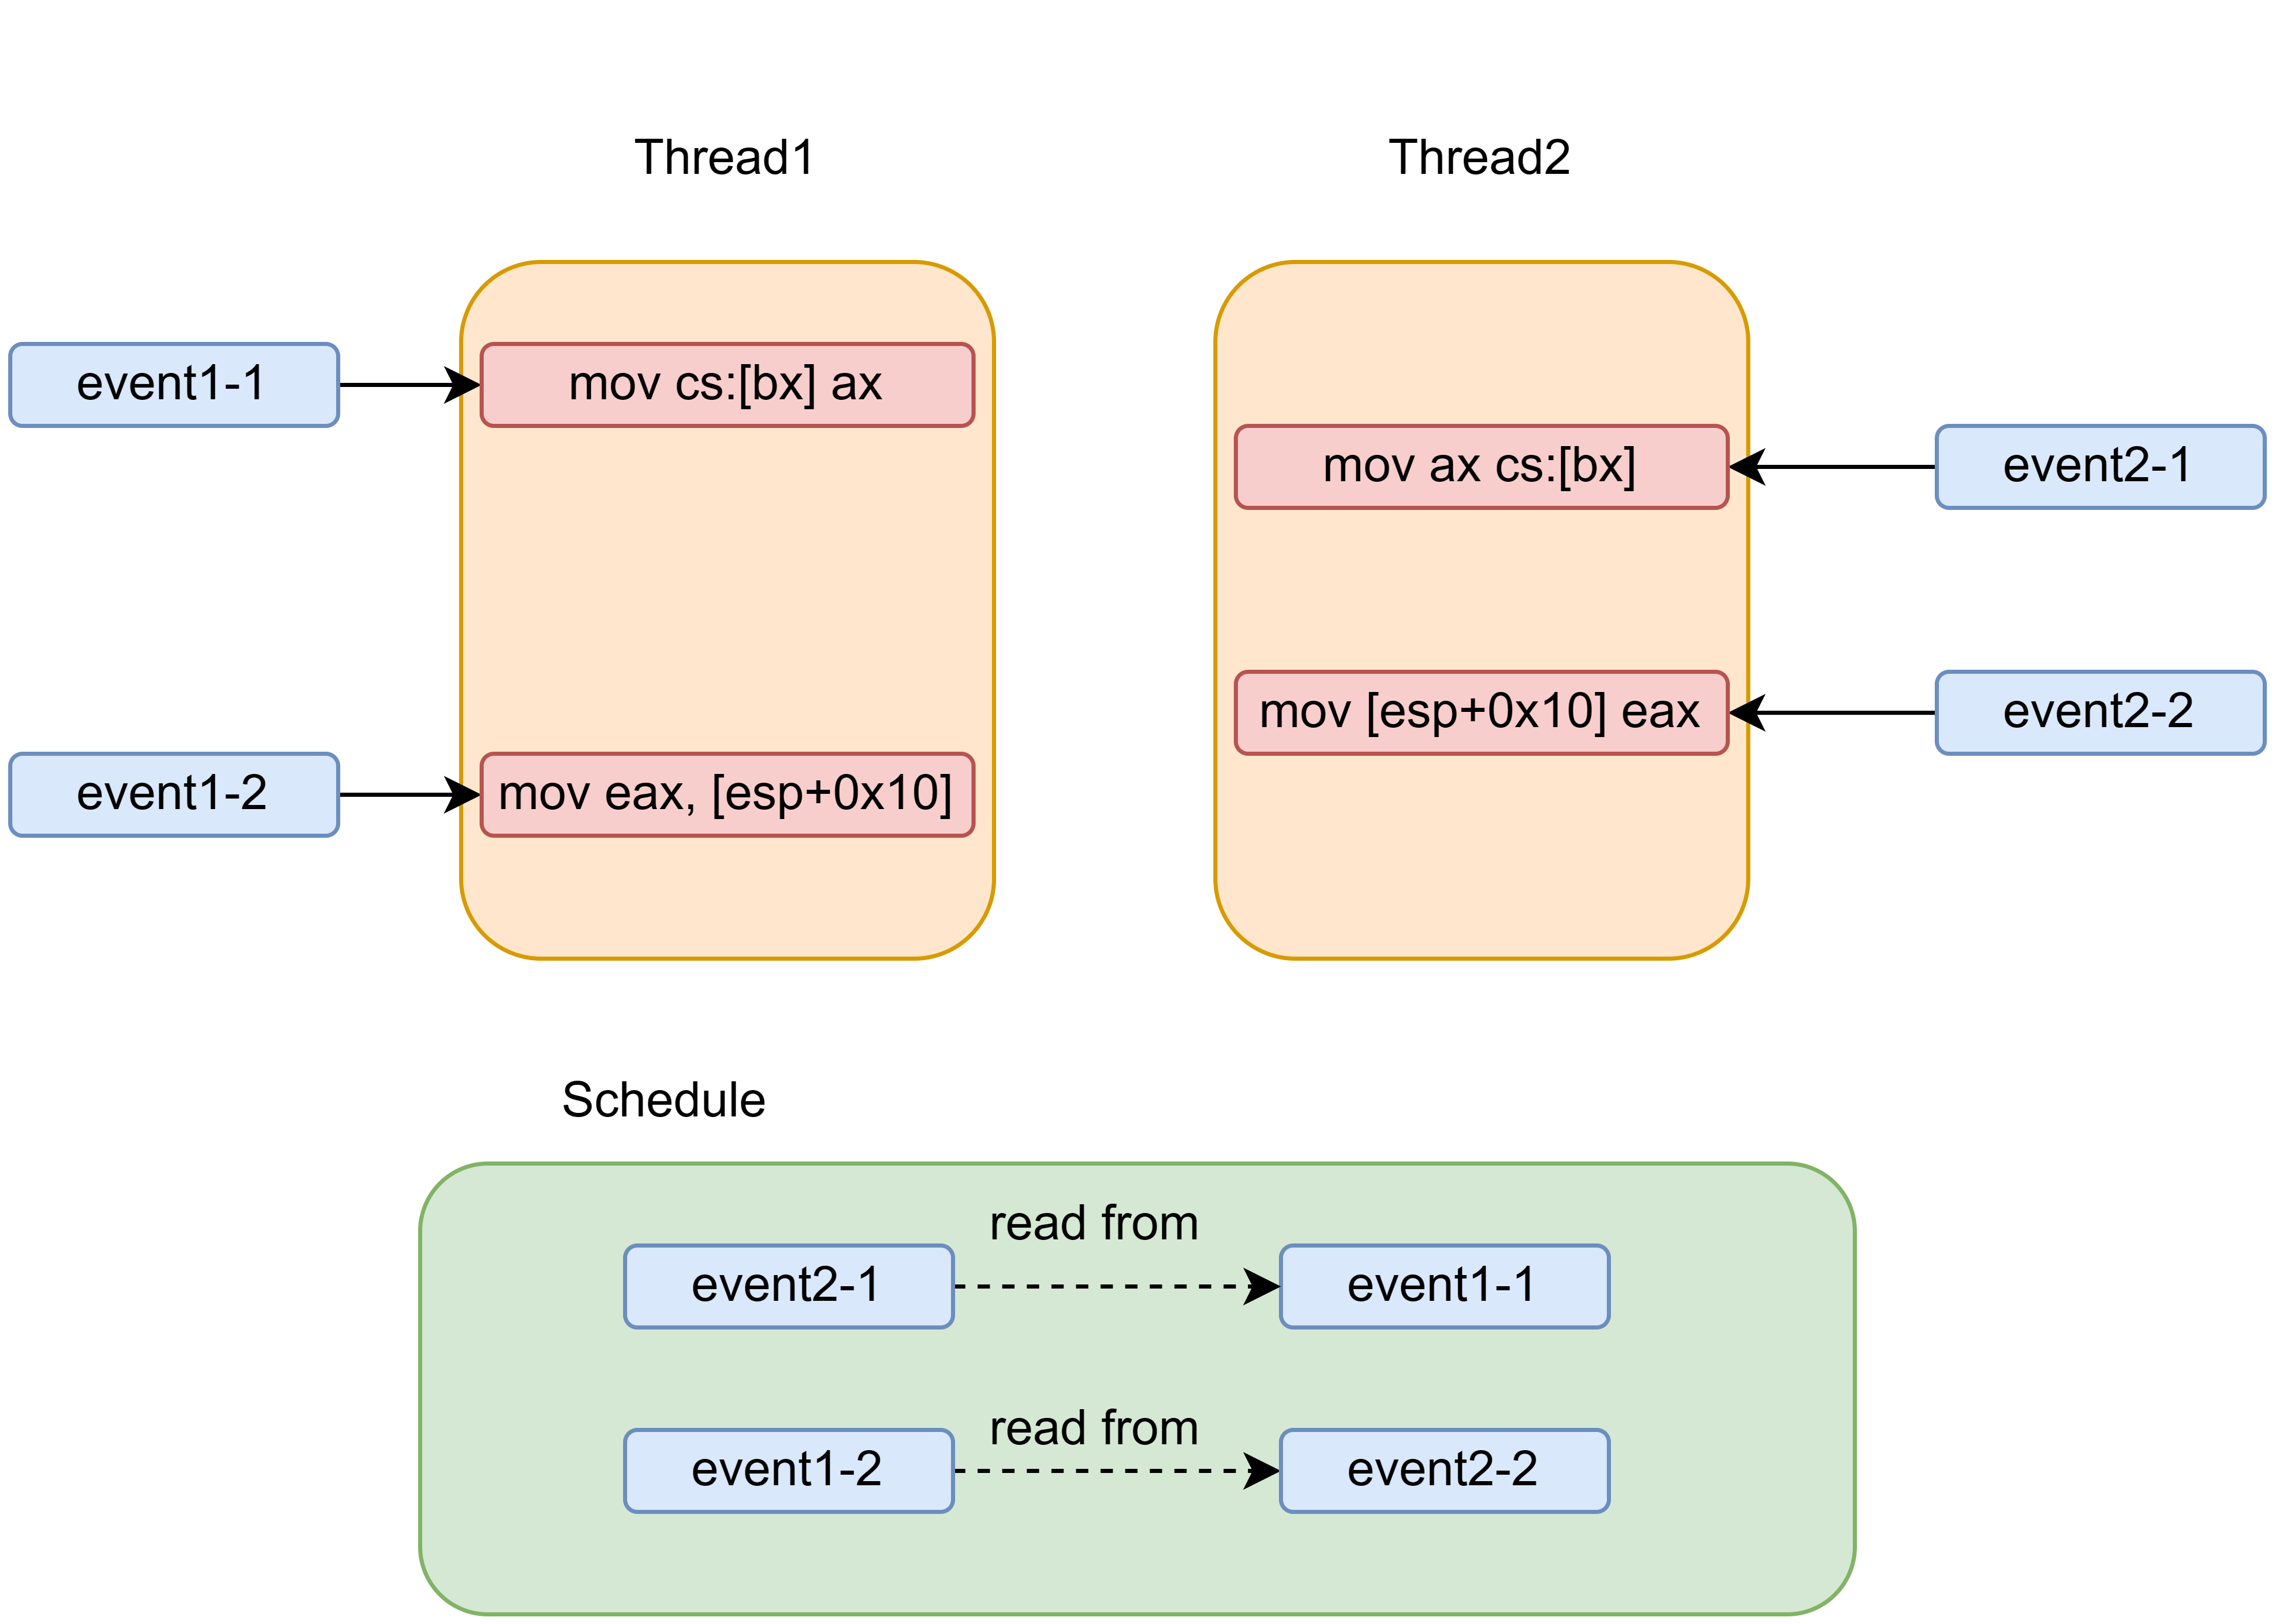
\includegraphics[width=.9\linewidth]{event_sche}
    \caption{\label{fig:event_sche}Event and Schedule}
\end{figure}

将reads-from relation作为基础构建等价调度集是合理的。首先我们在Section 2.1.1中提到过,竞争条件发生的根本原因是是由于读写错位导致的,所以说调整读写的顺序,也就能对不同的可能发生错误的情况进行尝试。在整个多线程程序运行的过程中,除了读和写的操作,其他的操作不会和其他线程产生交集,因此也不会造成并发的错误,这也是为什么reads-from relation没有对除了读和写之外的操作进行记录。

为了简单起见,这里首先分析两个操作的情况下为什么会产生并发错误。如果两个操作都是读的话,这种情况下并不会发生并发的错误,但是在两个操作中,有一个是写的操作时就会导致错误,比如说第一个操作对一个位置进行了写的操作,第二个位置原本想要读取这个地方的值,但是被写操作覆盖了,所以说现在他读到了错误的值。而reads-from relation就正好能够定义这种读取其他的操作所写的值的情况,不同的reads-from relation就正好对应不同的读取其他操作写值的情况,因此,利用reads-from relation定义不同的schedule是比较合适的。

\subsubsection{抽象事件和抽象调度}

再定义了reads-from relation以及等价调度之后,这篇文章进一步定义了抽象事件和抽象调度。用来对一整个等价的调度集合进行表示,一个抽象的调度就能够表示一整个等价调度的集合。同时,抽象调度是一种实际的数据结构,可以作为后续进一步实现变异操作的基础。

一个抽象事件是一个三元组$ea=<op, x, \rho>$,其中op表示读操作或者写操作,x表示操作的对象或地址,$\rho$表示操作代码的位置。一个抽象调度就是一系列的正向和反向reads-from约束。一个正向调度就是一对具有reads-from relation的抽象事件。正向和反向调度就分别代表了一个线程跳向另一个线程和跳回来的过程。一个具体的调度就是所有具体的事件进行排列的序列。当两个具体的调度同时符合一个抽象调度时,就说明这两个调度是等价的,那么就可以将它们,归到同一个类中,进而只需要测试他们中的一个,就可以代表这整个等价调度类。

正如前面所说,定义了抽象调度及其数据结构,就可以方便地对它进行变异。因为前面定义的抽象调度是一系列抽象事件的集合,因此只需要对抽象事件的顺序或数量等进行变异,就可以进一步改变抽象调度。在文章中定义了四种变异的方式,分别是插入,交换,删除以及反向。文章的$mutate\_schedule$函数首先选取一种变异的方式,然后随机选取存在潜在矛盾的抽象事件,然后对这些矛盾的抽象事件进行变异到得到新的抽样调度,并且会保证新产生的抽象调度不会和前面的重复。

\subsubsection{Reads-from反馈和调度实现}

本篇文章除了使用通常灰和模糊测试所使用的控制流反馈,还使用了With from信息,作为并发探索空间的反馈。 当变异后的调度中包含其他之前调度都没有的新的reads-from关系,或者一个调度导致了程序崩溃,算法就会认为这个调度是有趣的,并加入到种子集合中。并且在每次选取种子时,模糊测试器还会进一步将探索的方向偏移到那些很少出现的with from约束的调度上去。

在产生了前面的抽象调度之后,模糊测试器需要利用这个调度在实际的运行时进行操作,实际的操作就是通过维持一个当前可运行指令的状态图,这个状态图通过指定相应操作的优先级来保证对应指令是否能够运行。例如对于一个特定的reads-from constraint,如果写操作和读操作都就绪,那么将读操作的优先级调低,保证先进性写操作,在进行读操作。在写操作完成之后,将读的优先级调高,并将其他对该地址写的操作的优先级调低,这样就可以保证能够按照调度的方序来运行相应的指令。这是一种稳定的实现调度的方式,能够保证在多线程的情况下,程序仍旧按照指定的运行顺序进行运行,避免了不确定性。同时,尽可能保证了低开销。

\subsubsection{工具架构与实现}

\begin{figure}[ht]
    \centering
    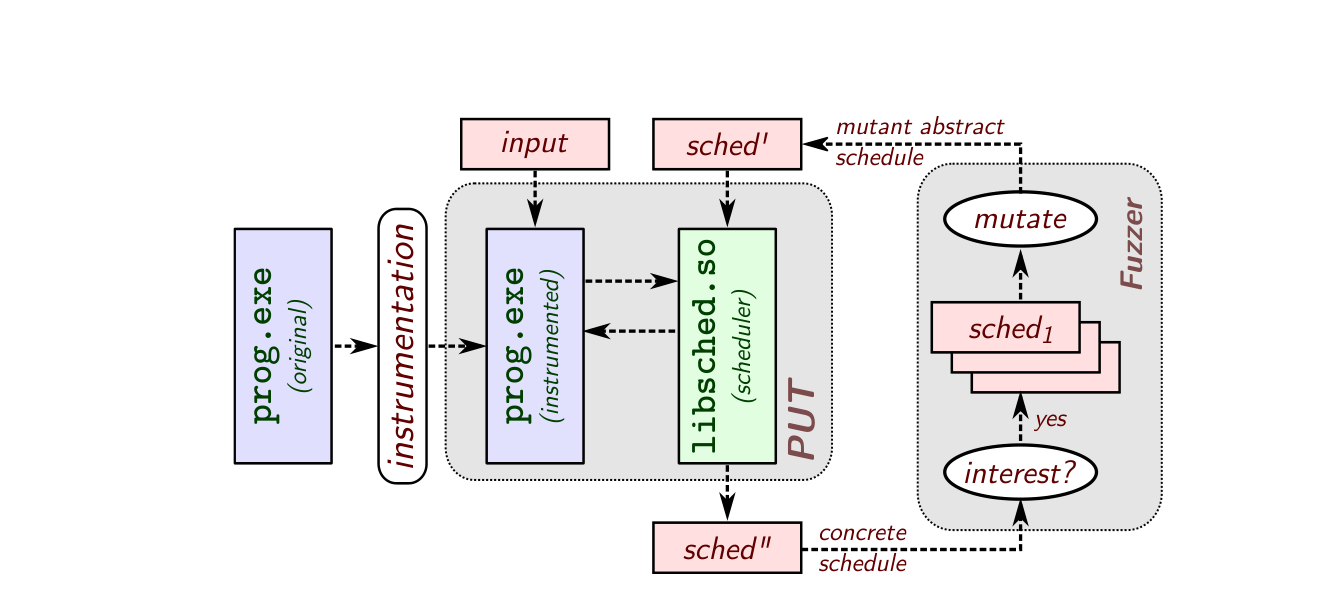
\includegraphics[width=\linewidth]{rff}
    \caption{\label{fig:rff}RFF Arhitecture}
\end{figure}

本篇文章复现了rff工具主要分为两个部分,第一个部分是用于对原始程序进行插桩,并得到可以被模糊测试器执行并获取运行必要信息的程序,以及一个确定性的用户态调度器。要二个部分是一个模糊测试器,基于AFL进行修改。RFF会对前面的程序分析,并生成一系列的种子,这些种子被视为是有趣的,即可能会导致并发漏洞的线程调度。在模糊测试的每一轮中,模糊测试期会对前面的有趣的种子进行变异来得到新的种子,并对这些种子进行排序,得到最有可能产生并发漏洞的种子,将其作为下一轮测试的输入。每一个输入都包含着一系列的reads-from relation。然后被插桩的程序在确定性用户调度器的操作下运行,调度器根据事件的约束生成相应操作的状态,只有在达到特定状态时才可以运行相应的操作,这样就实现了不同线程之间的调度。

\begin{spacing}{1.0}
\begin{lstlisting}[%
    language={C},
    caption={event.c},
    label={code:on_event},
]
void on_event(event_t id) {
    mutex_lock (& GLOBAL);
    thread_t *T = schedule(id);
    if (T != self()) {
        cond_signal (&T->wake);
        cond_wait (&self()->wake , &GLOBAL);
    }
    record(self(), id);
    mutex_unlock (& GLOBAL);
}
\end{lstlisting}
\end{spacing}

\paragraph{利用插桩实现基于锁的同步}首先在原始程序的处理阶段,RFF会分析原始程序并得到所有的event(内存操作,并发原语等),然后对这些操作进行插桩,在他们的前面插入一个$on_event$\autoref{code:on_event}函数,这个函数会使用一个互斥锁GLOBAL来线性化所有的线程。具体来说,每一个线程都会被分配一个本地变量wake,来表示它当前是否可以运行。当执行到$on_event$函数时,这个函数首先会获取GLOBAL互斥锁,确保其他的线程不会在此时运行到$on_event$函数,然后$on_event$会调用schedule函数来得到下一个将会执行的线程并唤醒它,然后将当前的线程睡眠。这个过程需要一定的时间,会对程序的运行造成一定的负载,但是这个负载是可以接受的。

schedule函数选择下一个将会运行的线程的算法如下。首先会根据wake变量来得到所有的可执行线程,然后在所有可执行的线程中,选择那些满足当前抽象调度的线程,具体来说就是不会违反reads-from relation的线程,最后,如果有超过一个线程,满足前面的两个条件,那么就会根据POS来随机选择一个线程。如果没有线程可以运行,那么就证明检测到了死锁。



\paragraph{针对调度的模糊测试器}RFF的第二个部分是针对调度的模糊测试器,它基于AFL工具,利用了AFL的共享内存区域机制,能够在被测试程序以及模糊测试器本身之间进行高效的沟通。这里我们对AFL进行修改,使其能够对调度进行模糊测试,而非常规的输入。\ref{power}展示了模糊测试器主要行为的伪代码。这个算法首先需要一个初始的调度集合作为输入,在每一轮模糊测试的过程中,首先从当前的调度集合中选取一个调度出来,然后对它进行变异产生一个新的调度$\sigma_{mut}$,并将这个调度应用于实际的程序上进行测试,如果在运行的过程中程序崩溃或者发生了其他的错误,$\sigma_{mut}$就会被加入到会导致崩溃的调度集合中,这个集合会作为最终的输出。除此以外,如果模糊测试器检测到$\sigma_{mut}$会导致新的行为,那么这个调度会被加入到初始调度集合中,用于进行后续的模糊测试。

算法\ref{power}有一些需要注意的特点。首先。这个算法并不是像纯粹的随机采样算法那样,随机采样算法在测试的过程中不会改变种子集合,也就是用于产生输入的集合,但是本算法通过动态保存一个调度集合并不断向里面加入其他的调度,这将有助于RFF从之前的测试中得到经验,用来指导后面模糊测试的方向。其次,这个算法没有去尝试产生所有的调度集合,它只保存了一个子集,尽管这样可能是不完整的,但是正如概述中讲到的,真正能够导致并发漏洞的调度只占全部调度集合的一小部分,因此即使只保留了一个调度的子集,RFF仍然能够有效地进行探索,并且由于需要处理的调度数量比较少,反而会提高模糊测试的效率。算法中通过$isInteresting()$函数来确定究竟哪些调度才是有趣的并将它加入到调度集合里面。传统的模糊测试将代码覆盖率作为一个反馈指标来确定一个输入是否有趣,但是对于并发程序的模糊测试,代码覆盖率并不能有效地反应调度是否有效。RFF还通过$PickNextAndAssignEnergy$函数来让模糊测试的方向更加有效。

\begin{algorithm}[!ht]
% \renewcommand{\algorithmicrequire}{\textbf{Input:}}
% \renewcommand{\algorithmicensure}{\textbf{Output:}}
\caption{Algorithm 1}
\label{power}
\begin{algorithmic}[1]
    \REQUIRE  Initial corpus of schedules $S_{init}$; % input 的内容
    
    \STATE $S \leftarrow S_{init}, S_{fail} \leftarrow \emptyset$
    \IF {$S = \emptyset$} \STATE $S \leftarrow {\epsilon}$;
    \ENDIF
    \REPEAT
        \STATE $(\sigma, \eta) \leftarrow PickNextAndAssignEnergy(S)$
        \FOR {$i \in \{1, \cdots, \eta_{\sigma}\}$}
            \STATE $\sigma_{mut} \leftarrow mutateSchedule(\sigma, S)$
            \IF {$\sigma_{mut}\ crashes$} \STATE $S_{fail} \leftarrow S_{fail} \cup \{\sigma_{mut}\}$
            \ENDIF
            \IF {$isInteresting(\sigma_{mut}, S)$} \STATE $S \leftarrow S \cup \{\sigma_{mut}\}$
            \ENDIF
        \ENDFOR
    \UNTIL {timeout}
    \RETURN {$S_{fail}$}
\end{algorithmic}  
\end{algorithm}

\subsubsection{示例}

这里利用下面的代码示例\autoref{code:example}来说明前面提到的核心思想。这里面的主程序首先会产生n = 100个子线程,这100个线程都尝试去修改全局静态变量a和b,最后还有一个线程用来检查最终a和b的值是否正确。假设a和b的读取操作都是原子性的,那么,这个程序执行操作总数为$\frac{(3n+2)!}{(n+1)!(3!)^n(2!)}$,而总的线程交错数量为$\Sigma^n_{i=1}\frac{C_i^n(n+i+1)!(2n-i)!}{(n+1)!2^n}$。面对如此大的搜索空间,如果仅仅随机产生调度,那么能够发现bug的概率非常小,POS这个算法提供了一个概率上的保证,但是仍然只能以比较低的概率进行。

\begin{spacing}{1.0}
\begin{lstlisting}[%
    language={C},
    caption={example.c},
    label={code:example},{}
]
static int a = 0, b = 0;
void setThread() {
    a = 1;
    b = -1;
}
void checkThread() {
    if(!((a == 0 && b == 0) || (a == 1 && b == -1))){
        assert(0); // Bug found
    }
}
int main() {
    const int n = 100;
    std::vector<std::thread> st;
    for (int i = 0; i < n; ++i) {
        st.push_back(std::thread(setThread));
    }
    std::thread ct(checkThread);
    return 0;
}
\end{lstlisting}
\end{spacing}

\subsection{PERIOD}

\subsubsection{概述}

正如前文所提到的,当前利用模糊测试挖掘并发漏洞的研究已经有了通用的流程,但是对于一些关键的问题仍然没有解决。比如多线程交错空间往往很大,但是能够导致并发错误的调度往往只占其中的很小一部分。在这么大的空间中,找到那一小部分调度是一个很关键的问题。再比如,在实际运行程序进行测试的过程中,如何根据一个已有的调度信息去控制多线程程序,按照相应的调度运行。这篇文章主要针对其中的两个问题:

\begin{enumerate}
\item 在进行实际的多线程程序运行的时候,如何保证受控的程序调度?虽然目前已经有很多种方案被提出,比如通过插装来实现抢占,睡眠延迟,或者动态线程优先级的修改。但是这些调度技术有可能和原本程序中的同步原语产生冲突,进而导致其他问题。例如,通过插桩来引入抢占式同步,往往也是利用锁机制,在引入这些锁同步机制之后,新的程序有可能会产生死锁。而利用睡眠延迟来同步,可能会被其他事件打断而产生不可预测的后果,而且这种方式可能会造成比较大的时间开销,造成测试效率降低。
\item 如何有效的探索调度空间?正如前文所说,程序调度空间的大小是会随着程序中调度点的数量的增多而指数级增长。想要穷尽调度空间,往往是不现实的。现有的工作大多以随机或者系统的方式探索调度空间,但是随机探索只能保证发现错误的概率,而系统测试在有限的指令中进行探索,尽管如此,它所需要探索的空间仍然很大,会造成比较大的开销。
\end{enumerate}

\subsubsection{动态关键点切片}

这里首先应该定义关键点,关键点就是一个对变量的访问的操作,基于这些对变量的访问,将一个单线程的程序进行切片,然后把它们组合为多线程的这个执行顺序,在这个切片的边界是对一个变量的访问。这篇文章将每一个切片称作为一个period。这篇文章同样观察到,并发漏洞往往发生在不同线程对相同变量的访问,并且这两个访问都靠近于程序进行切换时,所以对同一个变量访问时进行线程切换且切换到的程序访问同一个变量是最有可能产生并发漏洞的。因此,period通过系统的探索不同的程序切片方式,进而构造出可能产生并发漏洞的关键点切片。

\begin{spacing}{1.0}
\begin{lstlisting}[%
    language={C},
    caption={period1.c},
    label={code:period1},
]
if(done);                                       //period1
++waiters;
mutex_lock(lock); 
if(!done) 
    done=1; 
mutex_unlock(lock); 
if(!--waiters){ 
    free(lock); 
    lock = NULL; 
} 
                            if(done)            //period2
                                return 0;
\end{lstlisting}
\end{spacing}

这种方式还有一个好处就是它可以挖掘更深层次的并发漏洞。并发漏洞在大多数情况下都只涉及几个指令的访问。但是,在少数情况下可能涉及多个访问。Period基于这种系统探索保留前缀切片,在后续的切片中进行继续的探索,从而能够更深层次的对程序的并发访问空间进行探索,挖掘到更深层次的漏洞。

例如多线程程序\autoref{code:period1}。其中对done这个变量进行了多次的访问,尽管对访问做了一定的保护,但是仍然有可能产生并发漏洞。PERIOD通过将period1进行拆分来找到可能的冲突切片。以对period1进行切片为例,PERIOD逐个将最后一条指令分到PERIOD3中去,然后如果切换的边界点正好同样是对done的访问,则视为一个有趣的切片,并对其进行进一步的探索。这里首先将$lock = NULL$分到period3,然后再将$free(lock)$也分到period3,直到$done = 1$被分配到period3。此时代码的交错为\autoref{code:period2}。由于此时thread2的代码执行路径变化的了,因此相应的代码段也产生变化。至此,PERIOD发现了一个新的关键点切片,在此基础上会对period2进行下一次的切片,并不断持续下去。注意这种方式不一定会导致状态爆炸,因为在探索的过程中,有很多情况被舍弃掉了。当线程切换上下文两个指令并不都是对同一个变量或地址的访问时,这种切片不会被period保留下来并进行进一步探索,只有在上下文的为关键点时period才会保留下来并进行进一步的探索。

\begin{spacing}{1.0}
\begin{lstlisting}[%
    language={C},
    caption={period2.c},
    label={code:period2},
]
if(done);                                       //period1
++waiters;
mutex_lock(lock); 
if(!done) 

                            if(done)            //period2
                            ++waiters;
    done=1;                                     //period3
mutex_unlock(lock); 
if(!--waiters){ 
    free(lock); 
    lock = NULL; 
} 
                            mutex_lock(lock); 
                            if(!done)
                            mutex_unlock(lock);
                            if(!--waiters){ 
                                free(lock); 
                                lock = NULL; 
                            }
\end{lstlisting}
\end{spacing}

\subsubsection{Periodical Executor}

这篇文章要解决的第二个问题是基于生成的调度,在实际测试程序时,将多线程程序的运行序列化。前面提到之前的工作,可能会和原本程序的机制产生冲突,进而导致不可预知的情况发生。这篇文章使用了周期性的执行机制,它基于linux的Deadline任务调度,通过在每一个key point点之前设置$sched_yield$函数,在执行到这个函数时,会将当前线程挂起并执行其他线程。PERIOD会分配一个生命周期,每个period的生命周期都足够长来覆盖任何period中的关键点。当生命周期结束时,一个周期的执行也就结束了。

这种机制为线程的同步引入了一种可靠的机制,因为它是依托于操作系统原本设计的机制,因此,在使用时可以调用操作系统的接口,依托于操作系统的健壮性,具有比较高的可靠性。

\subsubsection{PERIOD架构与实现}

给定一个拥有n个线程的并发程序,假设程序的常规输入已经被确定并给出,因此,唯一的不确定性就是多线程调度关系,不同的调度关系可能会导致代码执行不同的路径,进而导致不同部分的代码被执行,只有那些关键的部分代码被执行到,才有可能触发并发漏洞。Period将程序执行的路径中的指令抽象为动态关键点切片,动态关键点切片由一系列的元素组成,每一个元素都是一系列的关键点。DKPS天然就反映了有一些特殊指令(也就是关键点)是需要通过特殊的调度才能让它生效,Period就会用不同的调度系统的探索所有的切片。系统的工作流程如下\autoref{fig:period_arch}:

\begin{figure}[ht]
    \centering
    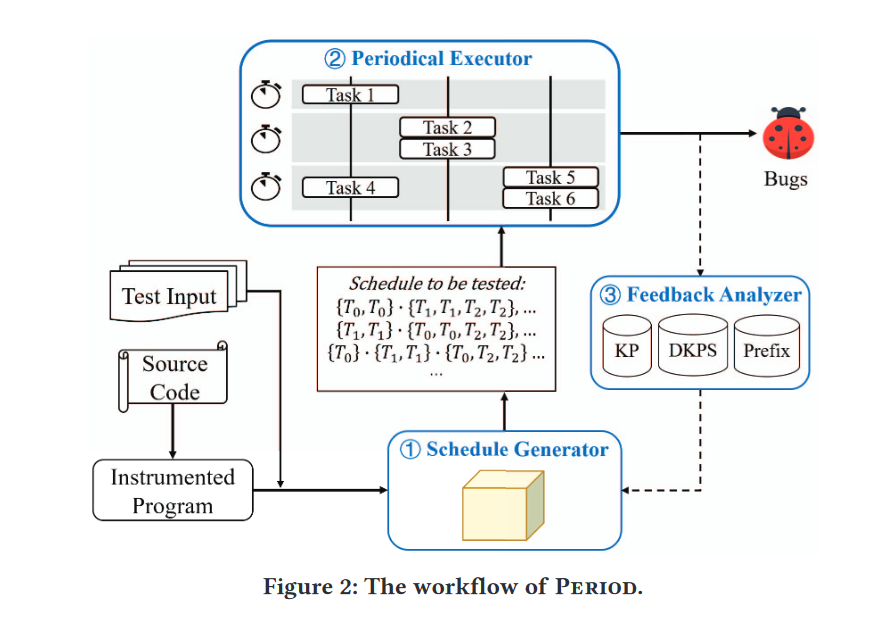
\includegraphics[width=\linewidth]{period_arch}
    \caption{\label{fig:period_arch}PERIOD Architecture}
\end{figure}

整个系统算法的设计如算法一所示,它的输入是一个待测的程序以及一个,预设的period界限,输出是一系列的bug以及它们对应的调度。在算法运行前,将会对待测试程序进行插装处理,以便在运行过程中获取必要的信息以及控制程序的调度。算法首先会产生一系列的jobs每个job对应一个线程,每一个job都包含一个d kps和一个调度前缀。调度前缀是为了记录前面的探索,并指导后面探索的方向。初始job的d kps只有一个关键点切片以及一个空的前缀调度。Period将会从只有一个切片开始,逐渐加深探索的深度,直到探索深度达到p位置。对于每一个Job以及每一个period数p,Period首先生成所有的调度,然后利用执行器测试所有的调度并记录是否产生bug。同时,执行器也会记录执行过程中产生的关键点切片信息,反馈分析器可以利用这些信息来决定是否应该产生一个新的job来探索对应调度的更深层。如果一个调度不是有趣的,或者说深度已经超过上限,那么这些Job就会被舍弃,不会再继续进行探索。

\begin{algorithm}[!ht]
% \renewcommand{\algorithmicrequire}{\textbf{Input:}}
% \renewcommand{\algorithmicensure}{\textbf{Output:}}
\caption{Algorithm 1}
\label{power}
\begin{algorithmic}[1]
    \REQUIRE  Initial corpus of schedules $S_{init}$; % input 的内容
    % \ENSURE $\mathbf{Q}$; % output 的内容
    需要根据具体的代码修改
    \STATE $S \leftarrow S_{init}, S_{fail} \leftarrow \emptyset$
    \IF {$S = \emptyset$} \STATE $S \leftarrow {\epsilon}$;
    \ENDIF
    \REPEAT
        \STATE $(\sigma, \eta) \leftarrow PickNextAndAssignEnergy(S)$
        \FOR {$i \in \{1, \cdots, \eta_{\sigma}\}$}
            \STATE $\sigma_{mut} \leftarrow mutateSchedule(\sigma, S)$
            \IF {$\sigma_{mut}\ crashes$} \STATE $S_{fail} \leftarrow S_{fail} \cup \{\sigma_{mut}\}$
            \ENDIF
            \IF {$isInteresting(\sigma_{mut}, S)$} \STATE $S \leftarrow S \cup \{\sigma_{mut}\}$
            \ENDIF
        \ENDFOR
    \UNTIL {timeout}
    \RETURN {$S_{fail}$}
\end{algorithmic}  
\end{algorithm}

\subsection{PCT}

\subsubsection{概述}

Probabilistic Concurrency Testing是一种用于挖掘并发漏洞的随机算法。和前面的方法类似,这种方法同样是尝试将可能的输入减少,达到提高效率的目的。具体来说,它通过给定的线程数量,步骤数量以及漏洞深度(能够发现漏洞的最小调度限制数量)来对交错空间进行探索。同时,利用随机生成的算法,在数学上证明可以以稳定的概率发现漏洞。

\subsubsection{基于动态优先级调整的随机算法}

PCT是一种可以以最低概率检测并发漏洞的方法,它是基于优先级的,首先,他会为每一个线程赋予一个不同的优先级,越小的数字代表越低的优先级。在运行的时候,调度器只有在所有其他高优先级线程都被阻塞的时候才会运行优先级小的线程。每次只有一个线程,会被调度器选择运行,一个线程可能会被等待资源等问题所阻塞。当线程在运行的过程中到达一个优先级改变点时,可以改变它的优先级。每一个这样的改变点,都预先有一个确定的优先级,当线程运行到改变点时,调度器将线程优先级改到事先确定好的那个优先级。

给定输入n(线程数量),k(总的指令数量),d(漏洞深度),PCT按照如下的步骤工作。

\begin{enumerate}
\item 随机将n个初始优先级的值$d, d+1, \cdots, d+n$赋给n个线程。(保留了$1,\cdots, (d-1)$,便于改变点使用,将线程优先级调得更低)
\item 在所有指令中选取$d-1$个随机的改变点$k_1, k_2, \cdots, k_{d-1}$。每一个改变点$k_i$都有一个关联的优先级值$i$。
\item 按照优先级来执行线程。当一个线程到达了相应的改变点$k_i$,将相应的优先级值$i$赋给对应的线程。然后调度器会决定下一个执行的线程并运行它。
\end{enumerate}

这里的随机调度器保证了\textbf{给定一个有n个线程、k条指令的程序,PCT可以以$\frac{1}{nk^{d-1}}$的最低概率发现深度为$d$的bug}

\subsubsection{PCT架构与实现}

\begin{algorithm}[!ht]
% \renewcommand{\algorithmicrequire}{\textbf{Input:}}
% \renewcommand{\algorithmicensure}{\textbf{Output:}}
\caption{Algorithm 1}
\label{power}
\begin{algorithmic}[1]
    \REQUIRE  Initial corpus of schedules $S_{init}$; % input 的内容
    % \ENSURE $\mathbf{Q}$; % output 的内容
    需要根据具体的代码修改
    \STATE $S \leftarrow S_{init}, S_{fail} \leftarrow \emptyset$
    \IF {$S = \emptyset$} \STATE $S \leftarrow {\epsilon}$;
    \ENDIF
    \REPEAT
        \STATE $(\sigma, \eta) \leftarrow PickNextAndAssignEnergy(S)$
        \FOR {$i \in \{1, \cdots, \eta_{\sigma}\}$}
            \STATE $\sigma_{mut} \leftarrow mutateSchedule(\sigma, S)$
            \IF {$\sigma_{mut}\ crashes$} \STATE $S_{fail} \leftarrow S_{fail} \cup \{\sigma_{mut}\}$
            \ENDIF
            \IF {$isInteresting(\sigma_{mut}, S)$} \STATE $S \leftarrow S \cup \{\sigma_{mut}\}$
            \ENDIF
        \ENDFOR
    \UNTIL {timeout}
    \RETURN {$S_{fail}$}
\end{algorithmic}  
\end{algorithm}

\subsubsection{示例}

但是当现在的数量超过两个的时候,最低的概率可能就不再是1/2,。因为在这种情况下,即使线程2的优先级比线程2更高,但是进程2可能因为需要获取锁或其他的情况,导致被线程3阻塞,而线程3优先级比线程1更低,那么在这种情况下,线程1就可能在线程2之前运行,也就导致无法触发并发漏洞的情况。但是当线程1的优先级为所有线程中最低时,无论线程2是否被其他线程阻塞,线程1都不可能在线程2之前执行。

当bug的深度超过1时,算法需要做更多的尝试来触发相应的漏洞。只有线程2在两个操作之间发生了优先级的改变,才有可能导致线程1的指令在线程2两个指令之间执行。那么,程序优先级改变点在线程2的两个指令之间的可能性为$\frac{1}{k}$,除此以外,还需要保证线程1在线程二2执行到第一条指令之前,都必须是最低的优先级,因此,找到这个并发漏洞的概率为$\frac{1}{nk}$。

第三种情况和第二种情况类似,只不过比第二种情况多了一次要求,即在第2个线程获取b锁和a锁之间需要改变优先级。

\begin{figure}[ht]
    \centering
    \includegraphics[width=\linewidth]{pct_example}
    \caption{\label{fig:pct_example}Bugs for Different Depth}
\end{figure}

\subsection{POS}

\subsubsection{概述}

\textit{Partial order sampling} (POS)是一种用于进行并发漏洞检测的方法,同样是基于优先级分配的事件调度,相比于Section3.3提到的PCT的随机采样方法,POS通过建模排序约束为二分图,并计算这些约束可通过随即优先级分配得到满足的概率,利用这些概率选取下一个event。

相比于之前的PCT,由于引入了排序约束,POS在随机生成的程序能检测到bug的最低概率比随机采样和PCT强134.1倍,在SCTBench这个测试集上检测到错误的速度比随机漫步和PCT快2.6倍。

\subsubsection{随机漫步以及PCT方法的不足}

\begin{figure}[ht]
    \centering
    \includegraphics[width=\linewidth]{pct_buzu}
    \caption{\label{fig:pct_buzu}展示PCT能力不足的例子}
\end{figure}

第一种随机漫步方法是指在每一步中随机选取一个启用的事件来执行,这种方法往往比穷举测试的效果要好,因为漏洞往往只占整个搜索空间的一小部分,因此系统的进行测试可能导致长时间无法涉及到漏洞相关的调度。但是随机漫步无法保证发现错误的概率。在\autoref{fig:pct_buzu}(a)中线程A的断言当且仅当线程B的$x = 1$在这个断言之前执行时才会触发断言错误。在不知道哪种顺序会触发失败的情况下,我们应该均匀地对两种顺序进行采样,因为这样检测错误的最小概率是两种顺序中的最小采样概率。但是当错误顺序只涉及到极少数的事件时,随机漫步可能产生非常不均匀的顺序采样。在这个例子中们为了触发故障,线程A的断言必须被延迟m次才能成功触发错误,这个概率是$\frac{1}{2^m}$。

第二种方法是\textit{probabilistic concurrency testing}(PCT),为了更加均匀地采样不同顺序,PCT依赖于用户提供的参数d,即延迟的事件数,随机在执行过程中挑选d个事件进行延迟,转到其他线程运行。由于事件是随机选择的,其对交错空间的探索是均匀的,其在概率上有更大的保证。再次参考\autoref{fig:pct_buzu}(a),为了触发断言错误,没有其他事件需要被延迟,只需要决定最初两个程序的优先级,因此触发的概率是$\frac{1}{2}$,这远高于$\frac{1}{2m}$。

但PCT并没有考虑到事件的偏序关系,因此其中有很多的冗余。如\autoref{fig:pct_buzu}(b)所示,如果没有考虑barrier()的效果,PCT会尝试延迟A1或者B1,但是这并不会对结果产生影响。除此以外,对于A2,B2,A3,B3这四个事件,PCT可能会尝试$A2 \rightarrow A3 \rightarrow B2 \rightarrow B3$和$A2 \rightarrow B2 \rightarrow A3 \rightarrow B3$两种交错方式,但是实际上这两种交错方式是等价的,因此造成了冗余测试,进而降低PCT的效率。

\subsubsection{POS框架与设计}

\begin{algorithm}[!ht]
% \renewcommand{\algorithmicrequire}{\textbf{Input:}}
% \renewcommand{\algorithmicensure}{\textbf{Output:}}
\caption{Algorithm 1}
\label{power}
\begin{algorithmic}[1]
    \REQUIRE  Initial corpus of schedules $S_{init}$; % input 的内容
    % \ENSURE $\mathbf{Q}$; % output 的内容
    需要根据具体的代码修改
    \STATE $S \leftarrow S_{init}, S_{fail} \leftarrow \emptyset$
    \IF {$S = \emptyset$} \STATE $S \leftarrow {\epsilon}$;
    \ENDIF
    \REPEAT
        \STATE $(\sigma, \eta) \leftarrow PickNextAndAssignEnergy(S)$
        \FOR {$i \in \{1, \cdots, \eta_{\sigma}\}$}
            \STATE $\sigma_{mut} \leftarrow mutateSchedule(\sigma, S)$
            \IF {$\sigma_{mut}\ crashes$} \STATE $S_{fail} \leftarrow S_{fail} \cup \{\sigma_{mut}\}$
            \ENDIF
            \IF {$isInteresting(\sigma_{mut}, S)$} \STATE $S \leftarrow S \cup \{\sigma_{mut}\}$
            \ENDIF
        \ENDFOR
    \UNTIL {timeout}
    \RETURN {$S_{fail}$}
\end{algorithmic}  
\end{algorithm}

% \subsection{RFF与其他工具的比较}